\chapter{Introducción a la Criptografía}
En este capítulo voy a introducir los objetivos y ataques de un criptosis-\\tema, los criptosistemas simétricos y los distintos modos de funcionamiento de estos, así como los criptosistemas asimétricos y el uso de estos  criptosistemas en las aplicaciones de mensajería.

\section{Objetivos de un criptosistema y posibles ataques}
Todo criptosistema se construye con la finalidad de cumplir una serie de objetivos así como de protegerse de unos ataques. A continuación voy explicar de cuales se trata.
La información de este apartado ha sido obtenida de \cite{apuntesCriptografia}.\\ 
\subsection{Objetivos}
Los objetivos que tiene que cumplir un criptosistema son los siguientes.
\begin{description}
	\item \textbf{Confidencialidad.} 
		 La información solo puede ser accesible por las entidades autorizadas. 
	\item \textbf{Integridad.} 
		La información no ha sido alterada en el envío.
	\item \textbf{Autenticidad.} 
		La información proviene de quién afirma haberla enviado.
	\item \textbf{No repudio.}  
		El emisario de una información no puede negar haber realizado tal envío.
\end{description}
\subsection{Ataques}
Para hablar de los ataques supondremos que se sigue el principio de \emph{Kerckhoffs}, el cual establece que el adversario conoce todos los detalles del criptosistema excepto la clave empleada.\\
Los posibles ataques son:
\begin{description}
		\item \textbf{Criptograma.} El adversario conoce el criptograma, es decir, el mensaje cifrado o un fragmento de este.
		\item \textbf{Mensaje Conocido.} El atacante conoce parejas mensaje/criptograma cifradas con una misma clave.
		\item \textbf{Mensaje escogido.} El atacante puede generar criptogramas para mensajes de su elección. Una vez obtenidas dichas parejas, trata de averiguar el mensaje correspondiente a un criptograma desconocido.
		\item \textbf{Mensaje escogido-adaptativo.} El atacante no solo puede generar parejas mensaje/criptograma a su elección, sino que puede hacerlo tantas veces como quiera realizando los análisis que considere oportunos.
		\item \textbf{Criptograma escogido y escogido-adaptativo.} Similar a los anteriores pero partiendo del criptograma, teniendo acceso a descifrar los criptogramas que desee, inicialmente o a lo largo del proceso. Lo que se busca en este ataque es la clave.
\end{description}

Una vez vistos los objetivos que tienen que cumplir los criptosistemas y los posibles ataques de los que pueden ser objeto, voy a explicar el uso de los criptosistemas simétricos y asimétricos en las aplicaciones de mensajería.\\

\section{Criptosistemas simétricos y asimétricos en las aplicaciones de mensajería}
Los criptosistemas simétricos y asimétricos conforman un elemento fundamental en las aplicaciones de mensajería. Criptosistemas de ambas familias se usan de manera conjunta para garantizar la confidencialidad, integridad, autenticidad y no repudio de los mensajes.\\
Los criptosistemas simétricos son utilizados para cifrar los mensajes. Esto es debido a su velocidad de cifrado, su uso reducido de recursos y su mejor manejo de grandes cantidades de datos.
Tienen el defecto de que si la clave es interceptada, el criptosistema es vulnerado y se pierde tanto la confidencialidad como la autenticidad de los mensajes. 
Para evitar esto se suele complementar con métodos seguros para el intercambio de la clave como puede ser el \emph{intercambio de claves Diffie-Hellman}.\\
Los criptosistemas asimétricos son muy utilizados para la firma y autentificación de los mensajes, garantizando de esta manera la seguridad de la aplicación y se complementan con cifrados simétricos a la hora de cifrar los mensajes para garantizar de esta forma una eficiencia mucho mayor. Ya que uno de los principales problemas que tienen es su complejidad algorítmica a la hora de cifrar y descifrar los mensajes.\\

\section{Criptosistema simétrico}
Un criptosistema simétrico es un criptosistema en el cual se utiliza una sola clave para cifrar y descifrar un mensaje o es necesario conocer la clave secreta para desencriptar un mensaje. La importancia para garantizar la seguridad de los criptosistemas simétricos reside en el secreto de la clave, mientras que el conocer el algoritmo utilizado no es tan importante como medida de seguridad. Es decir, lo importante es que el atacante no conozca la clave, mientras que conozca el algoritmo usado no lo es tanto. La información ha sido obtenida de \cite{apuntesCriptografia}.\\
Un criptosistema simétrico está formado por:
\begin{itemize}
	\item $\mathcal{M}$ el conjunto de los mensajes, elementos candidatos a ser encriptados.
	\item $\mathcal{C}$ el conjunto de los criptogramas o mensajes obtenido después del proceso de encriptar.
	\item $\mathcal{K} \subseteq \mathcal{K}_p\times\mathcal{K}_s$ el espacio de las claves, elementos que se utilizan para encriptar y desencriptar los mensajes. 
\end{itemize}
Un criptosistema simétrico viene definido por dos aplicaciones
$$E:\mathcal{K}_p\times\mathcal{M}\rightarrow\mathcal{C},$$
$$\mathcal{D}:\mathcal{K}_s\times\mathcal{C}\rightarrow\mathcal{M}.$$
tales que para cualquier clave $k_p \in \mathcal{K}_p$, existe una clave $k_s$ de manera que dato cualquier mensaje $m \in \mathcal{M}$,
$$
\mathcal{D}(k_s,E(k_p,m))=m.
$$
Fijada la clave $k_p \in \mathcal{K}_p$ y su correspondiente $k_s \in \mathcal{K}_s$ se definen las funciones de cifrado y descifrado como:\\
\begin{aligned}
	\center
	&$E_{k_p}:\mathcal{M}\rightarrow\mathcal{C},$\\
	&$E_{k_p}(m)=E(k_p,m),$
\end{aligned}
\begin{aligned}
	\center
	&$D_{k_p}:\mathcal{C}\rightarrow\mathcal{M},$\\
	&$D_{k_s}(c)=D(k_s,c),$
\end{aligned}


\subsection{Cifrados de bloque}
A continuación voy a introducir los cifrados de bloque, ya que estos son fundamentales a la hora de cifrar los mensajes en las aplicaciones de mensajería debido a su eficiencia. El cifrado de bloque más utilizado actualmente es el cifrado \textbf{Rindael AES}. La información ha sido obtenida de \cite{apuntesCriptografia}.\\
Los cifrados de bloque son criptosistemas de clave simétrica en los que la longitud de los bloques y claves es fija.\\
Este criptosistema se define
$$
	E:\mathbb{B}^K\times\mathbb{B}^N\rightarrow \mathbb{B}^N,
$$
$$
	D:\mathbb{B}^K\times\mathbb{B}^N\rightarrow \mathbb{B}^N,
$$
donde N es el tamaño del bloque y K es el tamaño de la clave.\\
Los cifrados tienen distintos modos de operación los cuales dependen solo del tamaño del bloque. Estos modos permiten garantizar la confidencialidad de los mensajes, si bien, no garantizan su integridad. La información para describir los modos la he complementado con \cite{bloquenuevo}.\\ 
Los distintos modos usados en los cifrados de bloque son:\\
\begin{itemize}
	\item \textbf{Electronic CodeBook}\\
	Modo en el cual para una clave dada, se le asigna un bloque de texto fijo cifrado por cada bloque de texto plano. Los pasos que se siguen para encriptar y desencriptar son:
	\begin{itemize}
		\item \textbf{\emph{Cifrado ECB}}
		\begin{description}
			\item Dividimos m en $m_{[1]}\dots m_{[l]}$ con $m_{[i]} \in \mathbb{B}^N$
			\item Para $i\in \{1,\dots,l\}$ hacer
			\begin{description}
				\item $c_{[i]} = E_k(m_{[i]})$
			\end{description}
			\item Devolvemos $c_{[1]}\dots c_{[l]}$
		\end{description}

		\item \textbf{\emph{Descifrado ECB}}
		\begin{description}
			\item Dividimos c en $c_{[1]}\dots c_{[l]}$ con $c_{[i]} \in \mathbb{B}^N$
			\item Para $i\in\{1,\dots,l\}$ hacer
			\begin{description}
				\item $m_{[i]} = D_k(c_{[i]})$
			\end{description}
			\item Devolvemos $m_{[1]}\dots m_{[l]}$
		\end{description}
	\end{itemize}
%\newpage
		\begin{figure}[htb]
			\centering
			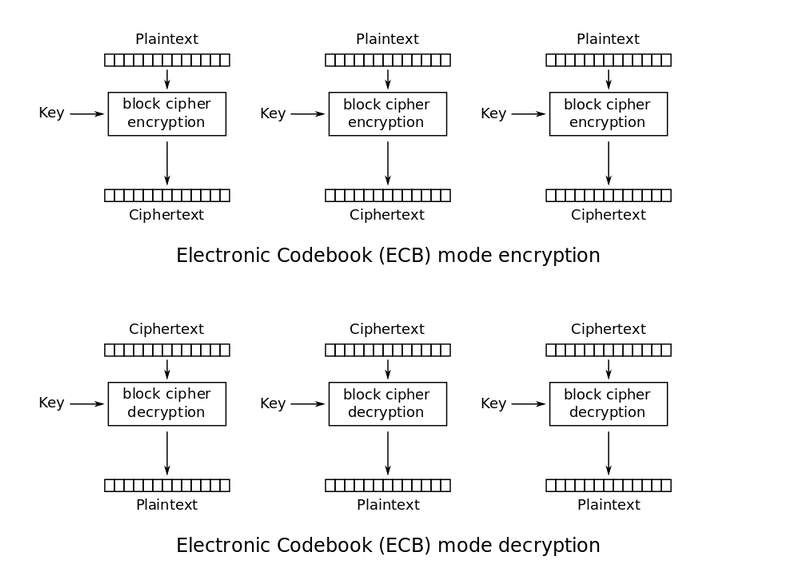
\includegraphics[scale=0.4]{imagenes/ecb.png} 
			\caption{Esquema del cifrado y descifrado del modo ECB \cite{cifradobloque}.}
			\label{esquemaecb}
		\end{figure}
		
	\item \textbf{Cipher-Block Chaining}\\
	En este modo se combina los bloques de texto plano con los bloques de texto cifrados anteriormente. Para cifrar el primer bloque será necesario un bloque inicial, $c_{[0]}$, el cual no tiene necesariamente que ser secreto. Los pasos seguidos para encriptar y desencriptar son:
	\begin{itemize}
		\item \textbf{\emph{Cifrado CBC}}
		\begin{description}
			\item $c_{[0]} \in \mathbb{B}^*$
			\item Dividimos m en $m_{[1]}\dots m_{[l]}$ con $m_{[i]} \in \mathbb{B}^N$
			\item Para $i\in\{1,\dots,l\}$ hacer
			\begin{description}
				\item $c_{[i]} = E_k(m_{[i]}\oplus c_{[i-1]})$
			\end{description}
			\item Devolvemos $c_{[1]}\dots c_{[l]}$
		\end{description}

		\item \textbf{\emph{Descifrado CBC}}
		\begin{description}
			\item Dividimos c en $c_{[0]}\dots c_{[l]}$ con $c_{[i]} \in \mathbb{B}^N$
			\item Para $i\in\{1,\dots,l\}$ hacer
			\begin{description}
				\item $m_{[i]} = D_k(c_{[i]})\oplus c_{[i]}$
			\end{description}
			\item Devolvemos $m_{[1]}\dots m_{[{l}]}$
		\end{description}
	\end{itemize}
\newpage
		\begin{figure}[htb]
			\centering
			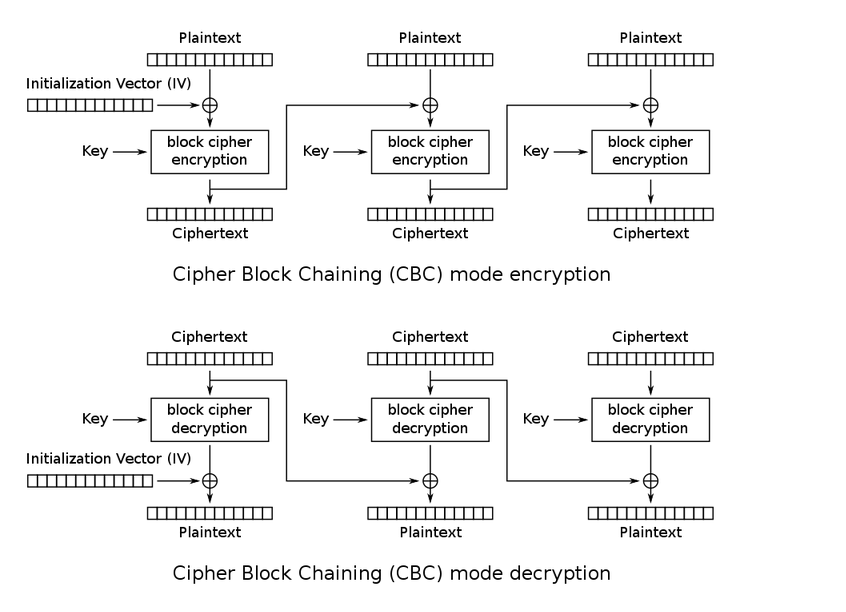
\includegraphics[scale=0.4]{imagenes/cbc.png} 
			\caption{Esquema del cifrado y descifrado del modo CBC \cite{cifradobloque}.}
			\label{esquemacbc}
		\end{figure}

	\item \textbf{Cipher FeedBack}\\
	Modo en el cual se combina cada bloque de texto plano del mensaje consigo mismo encriptado, los pasos que se siguen son:
	\begin{itemize}
		\item \textbf{\emph{Cifrado CFB}}
		\begin{description}
			\item $x_{[0]} \in \mathbb{B}^r$
			\item Dividimos m en $m_{[1]}\dots m_{[l]}$ con $m_{[i]} \in \mathbb{B}^N$
			\item Para $i\in\{1,\dots,l\}$ hacer
			\begin{description}
				\item $c_{[i]} = m_{[i]}\oplus msb_r(E_k(x_{[i]}))$
				\item $x_{[i+1]} = lsb_{N-r}(x_i)||c_{[i]$
			\end{description}
			\item Devolvemos $c_{[1]}\dots c_{[l]}$
		\end{description}

		\item \textbf{\emph{Descifrado CFB}}
		\begin{description}
			\item Dividimos c en $c_{[1]}\dots c_{[l]}$ con $c_{[i]} \in \mathbb{B}^r$
			\item Para $i\in\{1,\dots,l\}$ hacer
			\begin{description}
				\item $m_{[i]} = c_{[i]}\oplus msb_r(E_k(x_{[i]}))$
				\item $x_{[i+1]} = lsb_{N-r}(x_i)||c_{[i]$
			\end{description}
			\item Devolvemos $m_{[1]}\dots m_{[l]}$
		\end{description}
	\end{itemize}

%\newpage
		\begin{figure}[htb]
			\centering
			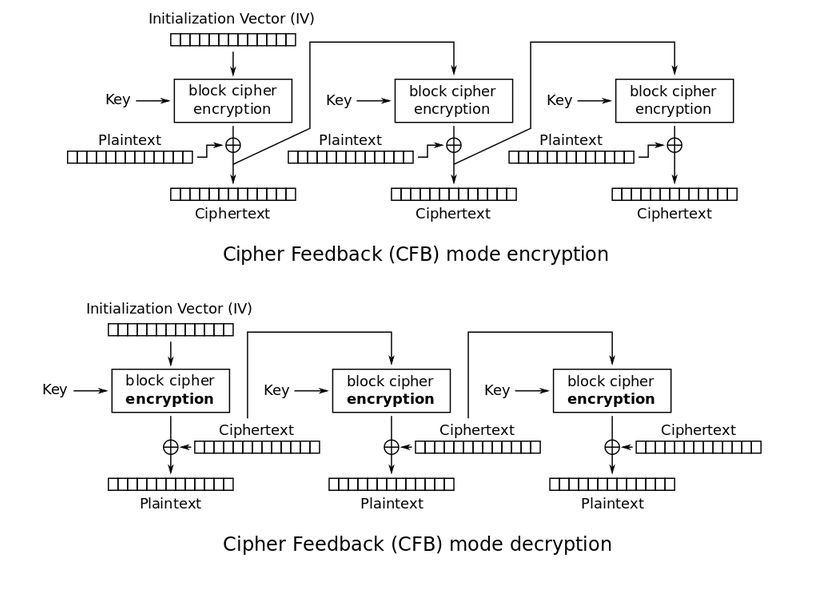
\includegraphics[scale=0.4]{imagenes/cfb.png} 
			\caption{Esquema del cifrado y descifrado del modo CFB \cite{cifradobloque}.}
			\label{esquemacfb}
		\end{figure}

\newpage
	\item \textbf{Output FeedBack}\\
	Modo en el cual se parte de un bloque inicial $x_{[0]}$ único y secreto. En cada iteración se encripta este y se combina con un bloque del mensaje sin cifrar de manera recursiva. Los pasos seguidos para encriptar y desencriptar son:
	\begin{itemize}
		\item \textbf{\emph{Cifrado OFB}}
		\begin{description}
			\item $x_{[0]} \in \mathbb{B}^N$
			\item Dividimos m en $m_{[1]}\dots m_{[l]}$ con $m_{[i]} \in \mathbb{B}^N$
			\item Para $i\in\{1,\dots,l\}$ hacer
			\begin{description}
				\item $x_{[i]} = E_k(x_{[i-1]})$
				\item $c_{[i]} = m_{[i]}\oplus x_{[i]}$
			\end{description}
			\item Devolvemos $c_{[1]}\dots c_{[l]}$
		\end{description}

		\item \textbf{\emph{Descifrado OFB}}
		\begin{description}
			\item Dividimos c en $c_{[1]}\dots c_{[l]}$ con $c_{[i]} \in \mathbb{B}^N$
			\item Para $i\in\{1,\dots,l\}$ hacer
			\begin{description}
				\item $x_{[i]} = E_k(x_{[i-1]})$
				\item $m_{[i]} = c_{[i]}\oplus x_{[i]}$
			\end{description}
			\item Devolvemos $m_{[1]}\dots m_{[l]}$
		\end{description}
	\end{itemize}
		\begin{figure}[htb]
			\centering
			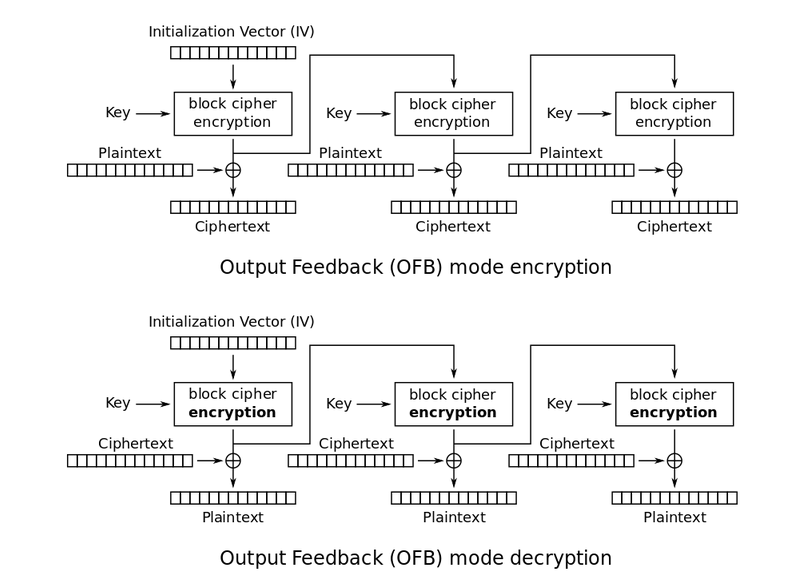
\includegraphics[scale=0.4]{imagenes/ofb.png} 
			\caption{Esquema del cifrado y descifrado del modo OFB \cite{cifradobloque}.}
			\label{esquemaofb}
		\end{figure}

\newpage

	\item \textbf{Galois Counter Mode (GCM)}\\
	Modo en el cual se usa un función hash universal sobre un cuerpo de Galois binario que provee de una autentica encriptación además de una método de validar los mensajes. La información de este modo ha sido obtenida de \cite{gcm}.
		Para cifrar en este modo partimos de una entrada con 4 elementos. 
		\begin{itemize}
			\item \emph{K} que es una clave secreta.
			\item \emph{IV} vector inicial que puede tener un número de bits entre 1 y $2^{64}$.
			\item \emph{M} texto plano que puede tener un número de bits contenido entre 0 y $2^{39}-256$.
			\item \emph{AAD} datos de autentificación adicionales, \emph{Additional Authenti-\\cated Data}, que puede tener un tamaño entre 0 y $2^{64}$ bits.
		\end{itemize}
		Y en la salida devuelve $C$ que es el texto encriptado y una autentificación $T$.\\
		Una vez visto la entrada y la salida, el algoritmo de cifrado y descifrado quedarían como sigue.
		\newpage
	\begin{itemize}
		\item \textbf{\emph{Cifrado GCM}}
		\begin{description}
			\item $H=E_k(0^{128})$
			\item Si $len(IV)=96$
			\begin{description}
				\item $Y_{[0]}=IV||0^{31}1$
			\end{description}
			\item si no
			\begin{description}
				\item $Y_{[0]}=GHASH(H,\{\},IV)$
			\end{description}
			\item Para $i\in\{1,\dots,n-1\}$ hacer
			\begin{description}
				\item $Y_{[i]}=incr(Y_{[i-1]})$
				\item $c_{[i]}=m_{[i]}\oplus E(Y_{[i]})$
			\end{description}
			\item $Y_{[n]}=incr(Y_{[n-1]})$
			\item $c_{[n]}=m_{[n]}\oplus MSB_u(E(Y_{[n]}))$
			\item $T=MSB_t(GHASH(H,A,C)\oplus E(Y_0))$
			\item Devolvemos $c=c_{[1]},\dots, c_{[n]}$ y $T$
		\end{description}
		Donde $A=A_1,\dots,A_m$, $incr(F||I)= F||(I+1\mod 2^{32})$ y la función $GHASH(H,A,C)$ equivale a calcular $X_{m+n+1}$. $X_i$ es una variable que se calcula como  
		
		\begin{equation}
		  X_i =
			\begin{cases}
				0 & \text{si } i= 0, \\
				(X_{i-1}\oplus A_i)\cdot H & \text{si } i\in\{1,\dots,m-1\}, \\
				(X_{m-1}\oplus(A_m||0^{128-v}))\cdot H & \text{si } i= m, \\
				(X_{i-1}\oplus C_i)\cdot H & \text{si } i\in\{m+1,\dots,m+n-1\}, \\
				(X_{m+n-1}\oplus(C_m||0^{128-u}))\cdot H & \text{si } i= m+n, \\
				(X_{m+n}\oplus(len(A)||len(C)))\cdot H & \text{si } i=m+n+1.
			\end{cases}       
			\notag
		\end{equation}\\

		\item \textbf{\emph{Descifrado GCM}}
		\begin{description}
			\item $H=E_k(0^{128})$
			\item Si $len(IV)=96$
			\begin{description}
				\item $Y_{[0]}=IV||0^{31}1$
			\end{description}
			\item si no
			\begin{description}
				\item $Y_{[0]}=GHASH(H,\{\},IV)$
			\end{description}
			\item $T^{'}=MSB_t(GHASH(H,A,C)\oplus(Y_0))$
			\item Para $i\in\{1,\dots,n-1\}$ hacer
			\begin{description}
				\item $Y_{[i]}=incr(Y_{[i-1]})$
				\item $m_{[i]}=c_{[i]}\oplus E(Y_{[i]})$
			\end{description}
			\item $Y_{[n]}=incr(Y_{[n-1]})$
			\item $m_{[n]}=c_{[n]}\oplus MSB_u(E(Y_{[n]}))$
			\item Devolvemos $m=m_{[1]},\dots,m_{[n]}$ y T'
		\end{description}
	\newpage
		Si T y T' coinciden entonces se devuelve el texto descifrado. Si no coinciden, entonces el texto no se devuelve ya que esto implicaría que el mensaje ha sido manipulado.
	\end{itemize}
		\begin{figure}[htb]
			\centering
			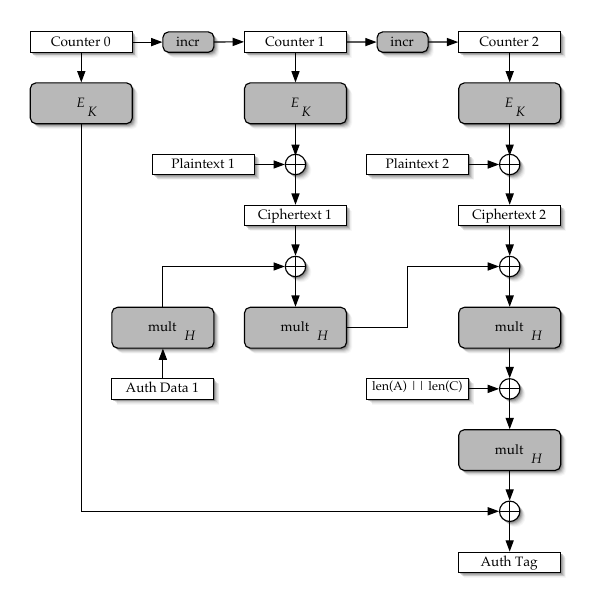
\includegraphics[scale=0.4]{imagenes/cgc.png} 
			\caption{Esquema del cifrado y descifrado del modo GCM \cite{gcm}.}
			\label{esquemagcm}
		\end{figure}
\end{itemize}
Como podemos ver, el modo más sencillo es ECB ya que lo único que hace es fragmentar el mensaje en bloques y encriptar individualmente cada bloque. En CBC, CFB, OFB y GCM se parte de un bloque inicial y se generan bloques nuevos de manera recursiva operando con ellos de manera distinta en función de cada modo.\\ 
En CBC se realiza la operación $\oplus$ de cada bloque generado encriptándose el bloque cifrado previo a esta con un bloque del mensaje, los nuevos bloques son los resultados de la operación anterior.\\
En CFB se coge el bit menos significativo resultante de encriptar el bloque generado previo y se hace la operación $\oplus$ con cada bloque del mensaje. Para generar un nuevo bloque se combina el mensaje cifrado previo con el bit menos significativo del conjunto de bits $N-r$ del bloque generado anterior con la operación $||$.\\
En OFB se realiza la operación $\oplus$ de el resultado de encriptar el bloque generado previo con un bloque del mensaje.\\
Y en GCM lo que se hace es fragmentar el mensaje y operar con los fragmentos de manera recursiva usando una función hash universal (\emph{GHASH}) con el primer bloque, además se realiza una operación paralela que se almacena en $T$ para certificar la integridad del mensaje.\\
Actualmente el más utilizado en las aplicaciones de mensajería es el modo CBC. Esto es debido a que es relativamente fácil de implementar y además permite encriptar en paralelo. Si bien, está empezando a utilizarse el modo GCM ya que implementado en hardware permite unas velocidades muy altas de encriptado llegando incluso a poder encriptar 10 GB por segundo. Un ejemplo de ello es la aplicación Line, que en su segunda versión incorpora este modo. 

\section{Criptosistema asimétrico}
Un criptosistema asimétrico es un criptosistema en el cual se utilizan dos claves, una para cifrar el mensaje y otra para descifrarlo. La clave para cifrar es la que se conoce como \emph{clave pública}, mientras que la que se utiliza para descifrar es la \emph{clave privada}. Estos criptosistemas surgieron para paliar la debilidad de los criptosistemas simétricos, que es que la clave que cifra y descifra se tiene que compartir, pudiendo esta ser interceptada.  
La seguridad de estos criptosistemas reside en que no se conozca la clave privada. La información ha sido obtenida de \cite{angelRiosMateos}.\\
Un criptosistema asimétrico está formado por:
\begin{itemize}
	\item $\mathcal{M}$ es el conjunto de los mensajes.
	\item $\mathcal{C}$ es el conjunto de los criptogramas.
	\item Una función $P:\mathcal{K}' \rightarrow \mathcal{K}$, que nos permitirá generar la clave pública. De manera que para cualquier clave privada $k' \in \mathcal{K}'$ obtenemos la clave pública como $P(k')=k$ 
\end{itemize}
Un criptosistema asimétrico viene definido por dos aplicaciones:
$$E:\mathcal{K}\times\mathcal{M}\rightarrow\mathcal{C},$$
$$\mathcal{D}:\mathcal{K}'\times\mathcal{C}\rightarrow\mathcal{M},$$
y se definen las funciones de cifrado y descifrado como:\\
\begin{aligned}
	\center
	&$E_{k}:\mathcal{M}\rightarrow\mathcal{C},$\\
	&$E_{k}(m)=E(k,m),$
\end{aligned}
\begin{aligned}
	\center
	&$D_{k^{'}}:\mathcal{C}\rightarrow\mathcal{M},$\\
	&$D_{k'}(c)=D(k',c).$
\end{aligned}

Para que un criptosistema asimétrico sea seguro tenemos que garantizar:
\begin{itemize}
	\item $P$ es una función de dirección única, es decir, que dado un elemento de su imagen no se puede calcular su imagen inversa fácilmente.
	\item Para la mayoría de los $k \in \mathcal{K}$, la aplicación $E_k$ es de dirección única.
	\item $\mathcal{D}_{k'}$ se puede calcular en un periodo corto de tiempo si se conoce $k'$ y es imposible o el periodo es muy largo en caso de solo conocerse $k$.
\end{itemize}
